\documentclass[]{article}
\usepackage{tikz}
%opening
\title{Example ARG and Recombination}
\author{Shaun Barker}

\begin{document}
	\begin{figure}[h!]
		\centering
		\begin{tabular}{c}
			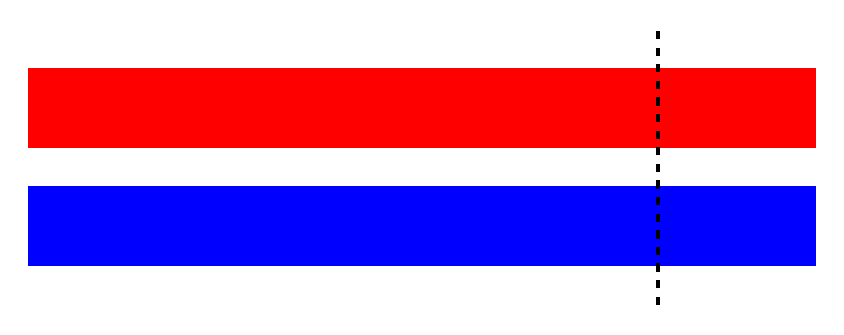
\begin{tikzpicture}
			\draw[color=blue,sharp corners, fill] (0,0) rectangle (10,1);
			\draw[color=red, sharp corners, fill] (0,1.5) rectangle (10,2.5);
			\draw[very thick,dashed] (8,-0.5) -- (8,3);
			\end{tikzpicture}\\
			Initially two parents have two separate genomes \\\\
			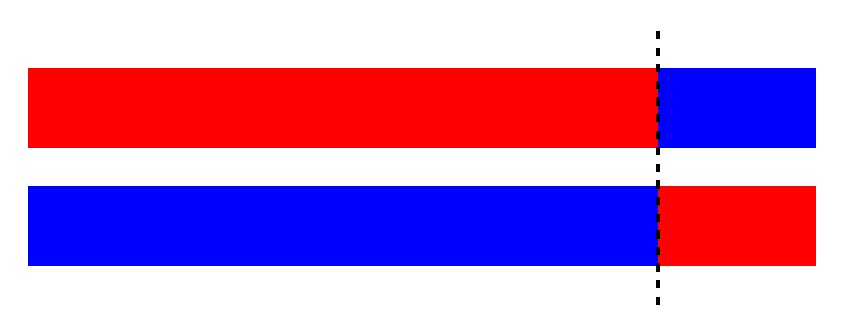
\begin{tikzpicture}
			\draw[color=blue,sharp corners, fill] (0,0) rectangle (8,1);
			\draw[color=red, sharp corners, fill] (0,1.5) rectangle (8,2.5);
			\draw[color=red,sharp corners, fill] (8,0) rectangle (10,1);
			\draw[color=blue, sharp corners, fill] (8,1.5) rectangle (10,2.5);
			\draw[very thick,dashed] (8,-0.5) -- (8,3);
			\end{tikzpicture}\\
			During reproduction their genes recombine in their offspring
		\end{tabular}
		\caption{A graphic demonstration the basic principles of recombination during reproduction using a red and blue genome}
		\label{recombinationForDummies}
	\end{figure}
	
	\begin{figure}[h!]
		\centering
		\begin{tikzpicture} [>=stealth]
		\draw[->, very thick] (-2,0) -> (-2,7) node[midway, anchor = south, sloped]{Time in the past};
		\draw (-1,0) -- (-1,2);
		\draw (2,0) -- (2,1) node[anchor=south]{0.4};
		\draw (6,0) -- (6,2) node[anchor=south]{0.3};
		\draw (5,2) -- (7,2);
		\draw (5,2) -- (5,3);
		\draw (1,1) -- (3,1);
		\draw (1,1) -- (1,2);
		\draw (-1,2) -- (1,2);
		\draw (0,2) -- (0,4);
		\draw (3,1) -- (3,3);
		\draw (3,3) -- (5,3);
		\draw (4,3) -- (4,4);
		\draw (7,2) -- (7,5);
		\draw (0,4) -- (4,4);
		\draw (2,4) -- (2,5);
		\draw (2,5) -- (7,5);
		\draw (4.5,5) -- (4.5,6);
		\end{tikzpicture}
		\caption{A simple ARG with three leaf nodes, two recombination events and four coalescent events that coalesce to a single branch in the past}
		\label{ARGexample}
	\end{figure}
	

\end{document}
